\documentclass[12pt]{article}
\usepackage{graphicx}
\usepackage {color}
\usepackage{pdfpages}
\usepackage{float}
\usepackage{changebar}
\usepackage{enumitem,amssymb}
\renewcommand{\familydefault}{\sfdefault}
\usepackage[margin=1.2in]{geometry}
\usepackage{graphicx}
\usepackage{wrapfig}
\usepackage[super]{cite}
\usepackage{subcaption}
\usepackage[table]{xcolor}
\usepackage{amsmath}
\usepackage[sort, numbers]{natbib}
\usepackage{multirow}
\usepackage{tabularx}
\usepackage{siunitx}

%%%%%%%%%%%%Defining the margins %%%%%%%%%%%%%%%%%%%%%
\textheight 9.in
\textwidth 6.5in
\topmargin -.5in
\oddsidemargin 0in
\setlength{\parskip}{\smallskipamount}

%%%%%%%%%%%%%%Specific Commands %%%%%%%%%%%%%%%%%%
\newcommand{\eg}{{\em e.g.,}}
\newcommand{\ie}{{\em i.e.,}}
\newcommand{\etc}{{\em etc.,}}
\newcommand{\etal}{{\em et al.}}
\newcommand{\degrees}{{$^{\circ}$}}
\newcommand{\fig}[1]{Figure~\ref{#1}}
\newcommand{\spo}{{SPO$_2$}}
%%%%%%%%%%%%%%%%%%%%%%%%%%%% Setting to control figure placement
% These determine the rules used to place floating objects like figures 
% They are only guides, but read the manual to see the effect of each.
\renewcommand{\topfraction}{.9}
\renewcommand{\bottomfraction}{.9}
\renewcommand{\textfraction}{.1}
\renewcommand{\familydefault}{\sfdefault} %setting the san serif font

%%%%%%%%%%%%%%%%%%%%%%%% Line spacing
% Use the following command for ``double'' spacing
%\setlength{\baselineskip}{1.2\baselineskip}
% and this one for an acceptable NIH spacing of 6lpi based on 11pt
%\setlength{\baselineskip}{.9\baselineskip}
% The baselineskip does not appear to work when we include a maketitle
% command in the main file.  Something there must set the line spacing
% If we use this next command, then things seem to work.
\renewcommand{\baselinestretch}{.9}

\setcounter{secnumdepth}{0} %make no numbers but have a table of contents


\begin{document}

\title{Lab 5: Exercise Stress}
\author{Jake Bergquist, u6010393, Partners: Bram Hunt, Katie Davis }
\maketitle

\section{Introduction}
In this laboratory exercise we set out to investigate the methodology by which blood pressure is measured externally, observe the various externally apparent features of the venous system, and investigate the effects of exercise on the parameters of blood pressure, heart rate, and ECG presentation. The ability to monitor blood pressure externally has been used diagnostically by physicians for many years. With the use of a blood pressure cuff and a stethoscope a physician can quickly assess the diastolic and systolic blood pressure using deflections of the pressure cuff and the sound of turbulent blood flow. Properties of the venous structure can also be characterized from external observation, such as the direction of flow and functioning of the valves. Our main goal was to utilize the blood pressure, and heart rate measures, along with a recorded ECG, to characterize the repose of the body to exercise. We chose to implement a model in which the subject either exercised intensely or moderately in short bursts followed by rest periods to characterize the response tot he exercise as well as the subsequent recovery. This investigation will show changes in ECG, blood pressure, and heart rate. We expect that blood pressure and heart rate should increase during exercise however the response may vary during sequential exercise periods. If the exercise is intense we expect that the parameters of blood pressure and heart rate will not be able to recover as well as when the exercise periods are moderate.


\section{Methods}

\subsection{Blood Pressure Measurement}
To assess blood pressure a blood pressure cuff was attached tot he left arm of the subject and inflated. The systolic pressure is first measured by inflating the cuff to block flow then slowly letting off low until the radial pulse returns by palpation. This also corresponds t a bump in pressure seen on the pressure gauge. The pressures were then taken again by inflating the cuff to cut of flow and a stethoscope was placed over the antecubital fossa. The pressure was released until a sound of blood flow returned (which was confirmed as the systolic pressure by the bump on the pressure gauge), and again until the sound stopped (diastolic pressure).

\subsection{Examination of Venous Function}
The subject was laid on the ground and a suitable set of veins was identified on the feet which were distinctly visible. The feet of the subject were raised above the heart until the point where they just barely collapsed. This distance was measured and used to calculate the venous pressure. A vein was then indentified on the hand of the subject and the flow was blocked manually.  The blood int he vein was then pressed towards and away from the block and released and the response was observed.

\subsection{Exercise Stress}
The subject was fit with four recording electrodes, one ont he left pectoral muslce (LA), one of the right pectoral muslce (RA), one on the left bottom of the rib cage between two ribs (LL) , one on the right bottom of the rib cage between two ribs (RL). RA, LA, and LL formed the standard limb lead configuration and RL served as a reference. Recording and exercise were performed according to Figure~\ref{fig:Protocol}. Before each phase a 30 second baseline ECG was taken along with a baseline hear rate, SP02, and blood pressure. In phase one the subject was instructed to peddle on the bike a maximu intensity (roughly 130 beats per minute on a metronome to time the pace of each peddle). Exercise was performed in 45 second intervals followed by 90 second rest periods. During the rest period blood pressure is measured as soon as possible, continuous ECG is recorded, and SP02 and heart rate are recorded every 10 to 15 seconds. Phase two is performed 30 minutes after phase one once the subject has fully recovered. Phase two follows the protocol of phase one witht he exception that the exercise intensity is reduced to be moderate with a pace of roughly 80 bpm for each pedal.

\begin{figure}[H]
	
	\centering
	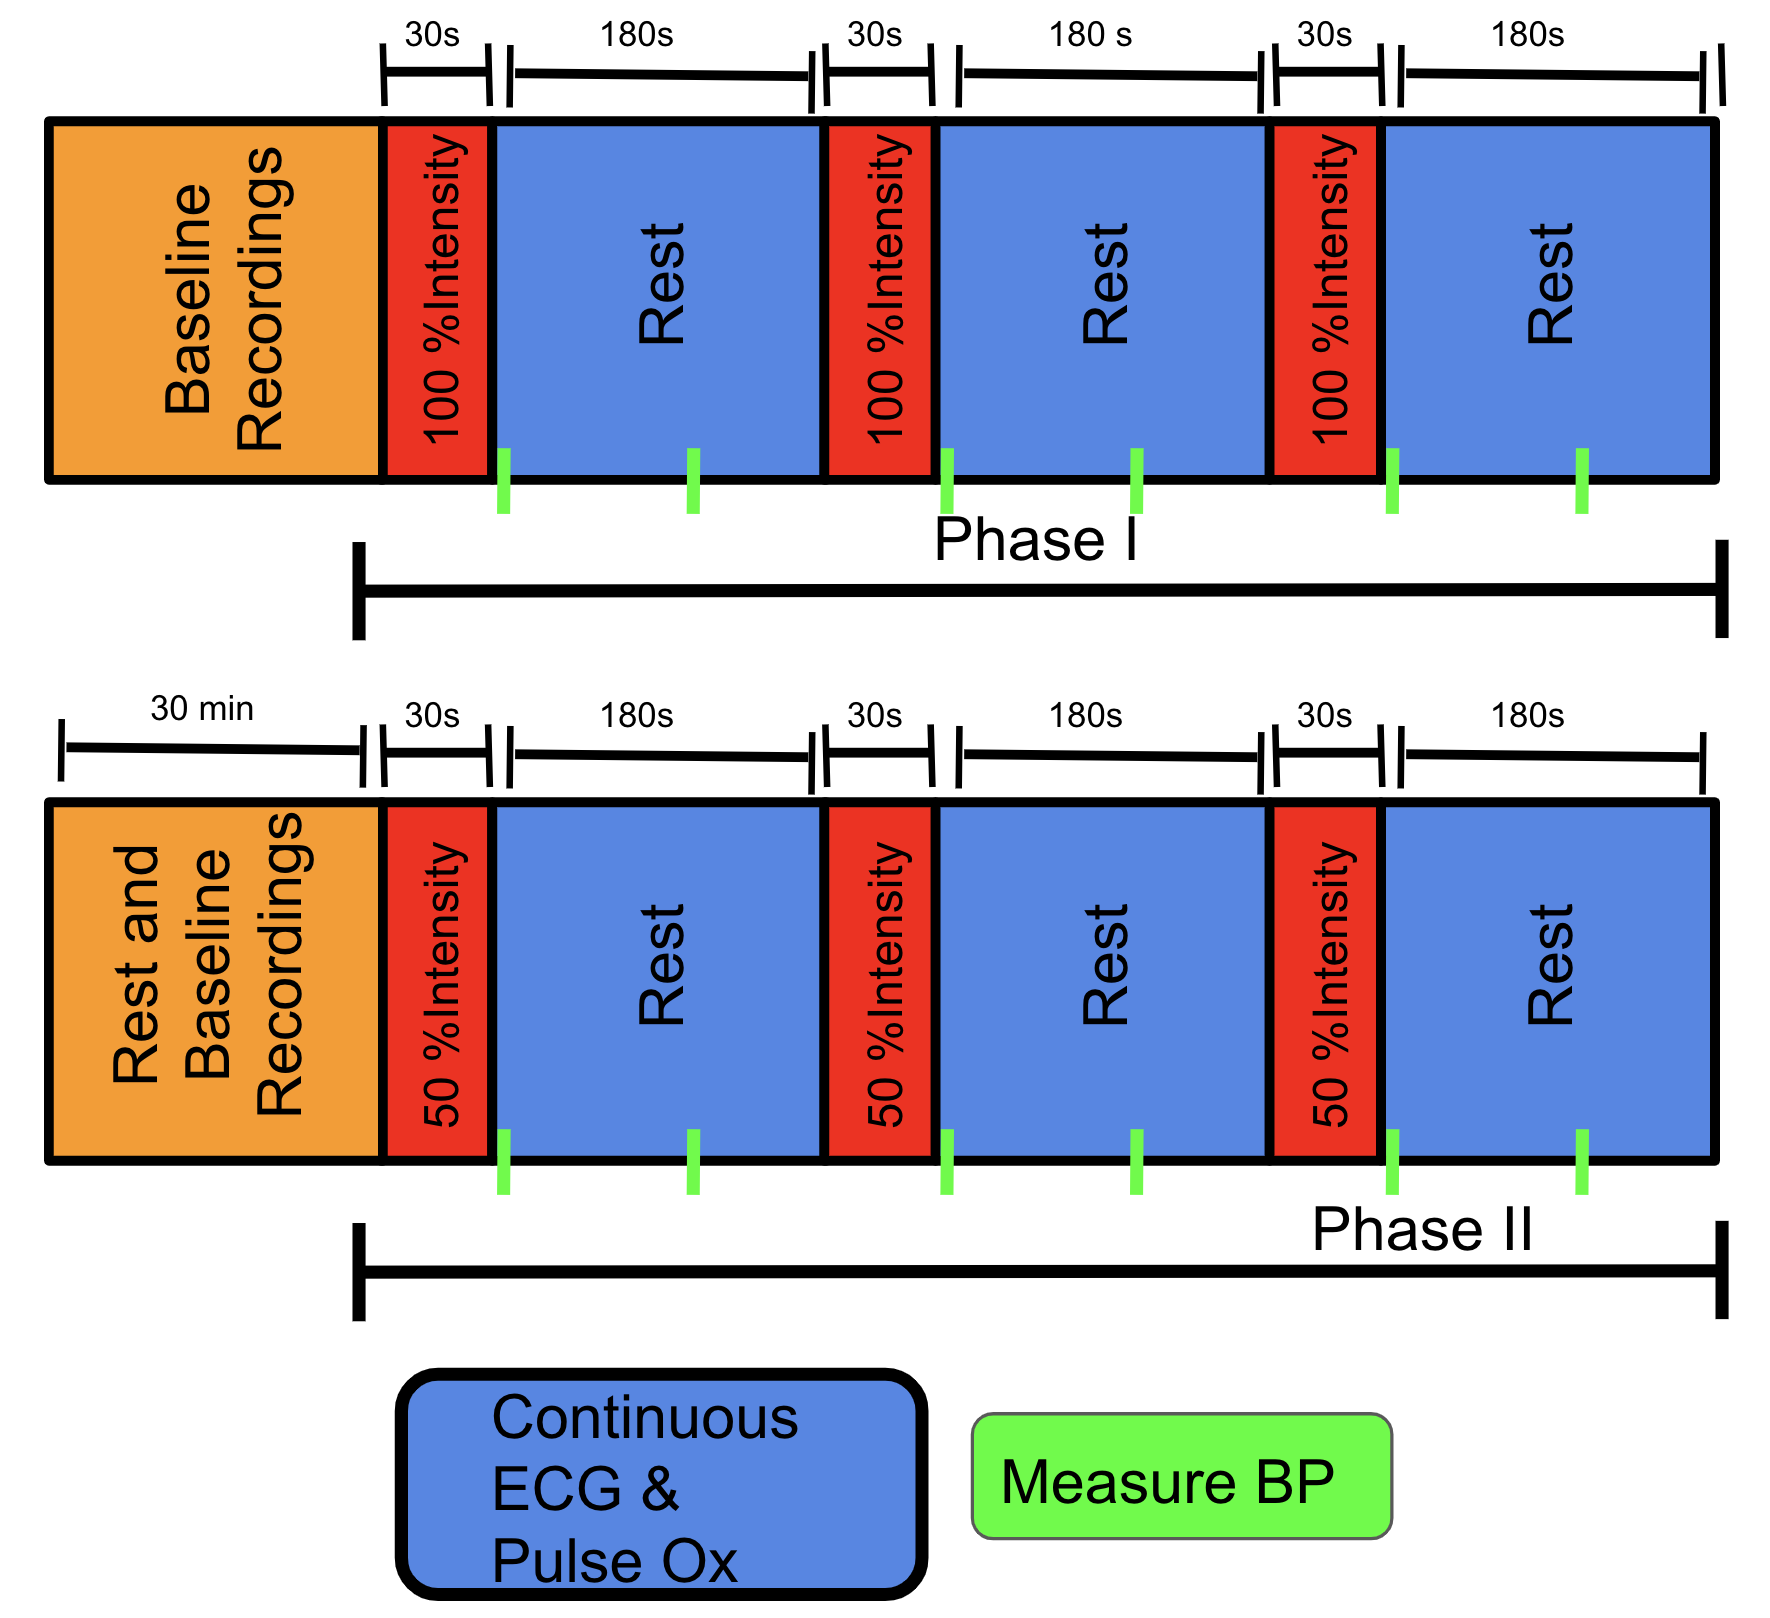
\includegraphics[width = .8\textwidth]{Figures/protocol.png}
	\caption{The designed exercise protocol. During phase I the subject were perform short bouts (30 seconds) of intense exercise (roughly 130 bpm pedal rate) followed by  180 second rest periods. Continuous ECG will be taken dsuring the rest periods as well as periodic \spo{}, BP, and heart rate measures. Phase II  will follow a 30 minute rest period and will be identical to phase I with the exception of the exercise being moderate (roughly 80 bpm pedal rate). Baseline recordings are taken before each phase.)}
	\label{fig:Protocol}
\end{figure}

\subsection{Processing}
The recorded ECG data was processed using PFEIFER, a preprocessing framework for electrograms, that filters, baseline corrects, fiducilizes, auto fiducilizes, and time aligns the signals.\cite{MacLeod2018_p} The time aligned baseline signals were averaged to produce cleaner signals. This was done by clustering similar beats using the kmeans clustering algorithm (MATLAB), and averaging these signals. The same process was performed for the first 5 and last 5 beats of each exercise protocol to produce signal averaged post experiment and post rest signals. Signals were assessed for qualitative differences during each recovery period and interesting changes were highlighted in the results.

\section{Results}
Using the palpatory method we measured a systolic blood pressure of 110 mmHg. Utilizing the Auscultatory method we could not quite distinguish when the non laminar sounds (Korotkow's sounds) started and stopped, however we were able to take the combined method measurements. This produced a systolic (when radial pulse returns) pressure of 110 mmHg, and a diastolic (first sound of Korotkow's sounds) pressure of 85 mmHg.

During the investigation of the venous system we measured the height at which the veins int he subject's foot just began to collapse. This was found to be 17 mm. Given the specific gravity of blood (1.056 g/mm) we get a value of around 1.32 mmHg for the venous pressure. When we pressed the blood in a vein back towards the valve we observed that the vein bulged and the blood was prevented from flowing in retrograde.

Before either exercise protocol the resting heart rate was 84 bpm and the \spo{} was 98\%. The baseline blood pressure was 110/85. Throughout the entire phase I and II the blood pressure remained elevated at 120/80 - 120/90. During  the 30 minute rest phase the blood pressure dropped to 110/75 but returned to the 120/80 range after the first phase II exercise protocol.

In Figure~\ref{HR} we see the heart rate for each recovery period. As can be seen for Phase I (solid lines) the heart rate starts at a higher level than the starting heart rate for phase II (dashed lines). In each case the heart rate drops rapidly at the onset of the rest periods and continues to drop throughout the rest periods. 

\begin{figure}[H]
	
	\centering
	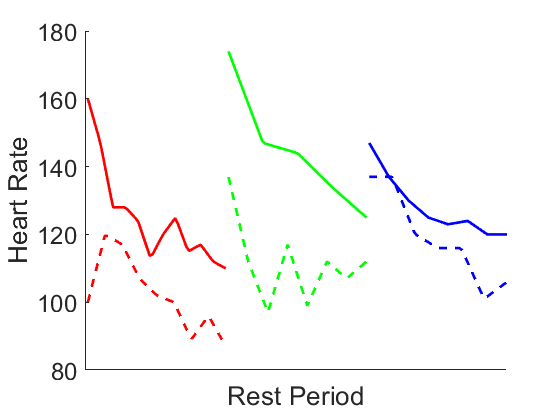
\includegraphics[width = .8\textwidth]{Figures/HR.png}
	\caption{Heart rate during each recovery period. Red: recovery period 1, green: recovery period 2, blue: recovery period 3. Solid lines from phase I, dashed from phase II.}
	\label{HR}
\end{figure}

The Oxygen saturation levels for each rest period are displayed in Figure~\ref{spo}. As can be seen the oxygen saturation did no fluctuate heavily during any rest period or across rest periods and phases of tyher experiment. The only notable exception is Phase I, recovery period 1 (red solid line) that had a slightly higher average \spo. 

\begin{figure}[H]
	
	\centering
	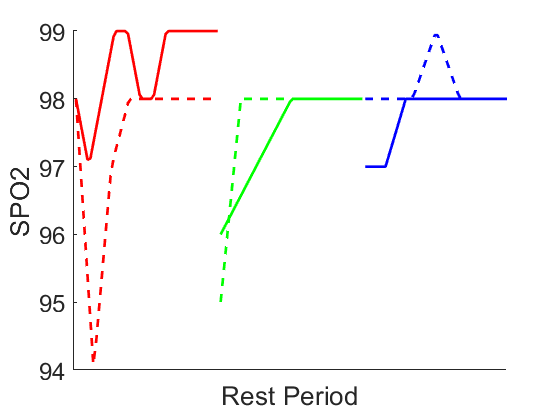
\includegraphics[width = .8\textwidth]{Figures/spo2.png}
	\caption{\spo{} during each recovery period. Red: recovery period 1, green: recovery period 2, blue: recovery period 3. Solid lines from phase I, dashed from phase II.}
	\label{spo}
\end{figure}

The signal averaged baseline ECG signals are shown in Figure~\ref{base} for each of the three limb leads. As can be seen the Phase II signals (dashed lines) are of a much higher amplitude. In Figure~\ref{exer} we see the signals from each limb lead immediately after exercise ceases with Phase I in solid lines and Phase II in dashed lines. Like the differences between baselines we see a similar increase in amplitude between Phase I and II. Finally Figure~\ref{reco} shows the signals at the end of each rest period before exercise was resumed. 

\begin{figure}[H]
	
	\centering
	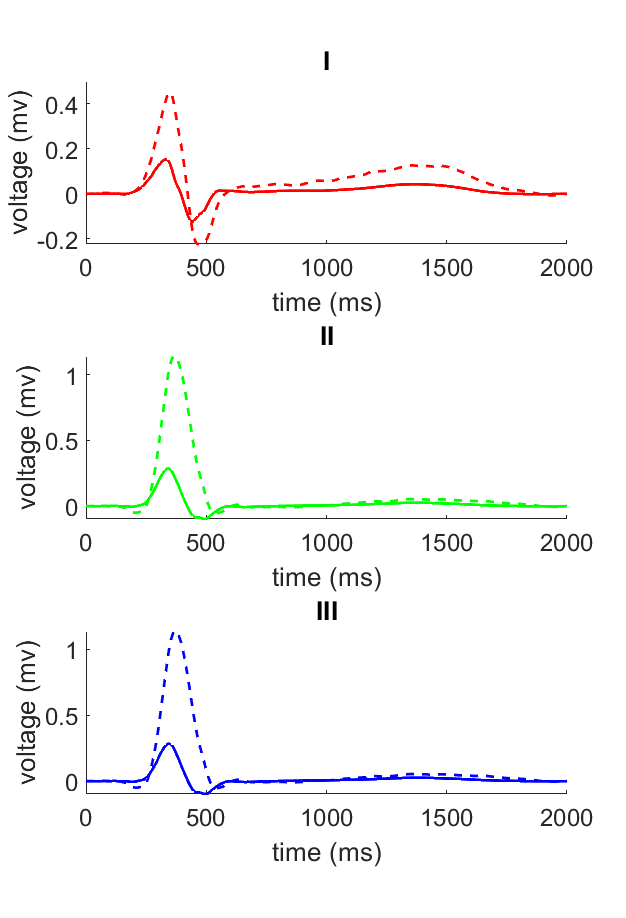
\includegraphics[width = .8\textwidth]{Figures/baselines.png}
	\caption{Baseline ECG. Red: lead I, green: lead II 2, blue: lead III. Solid lines from phase I, dashed from phase II. Signals were signal averaged from a continuous 30 second recording.}
	\label{base}
\end{figure}

\begin{figure}[H]
	
	\centering
	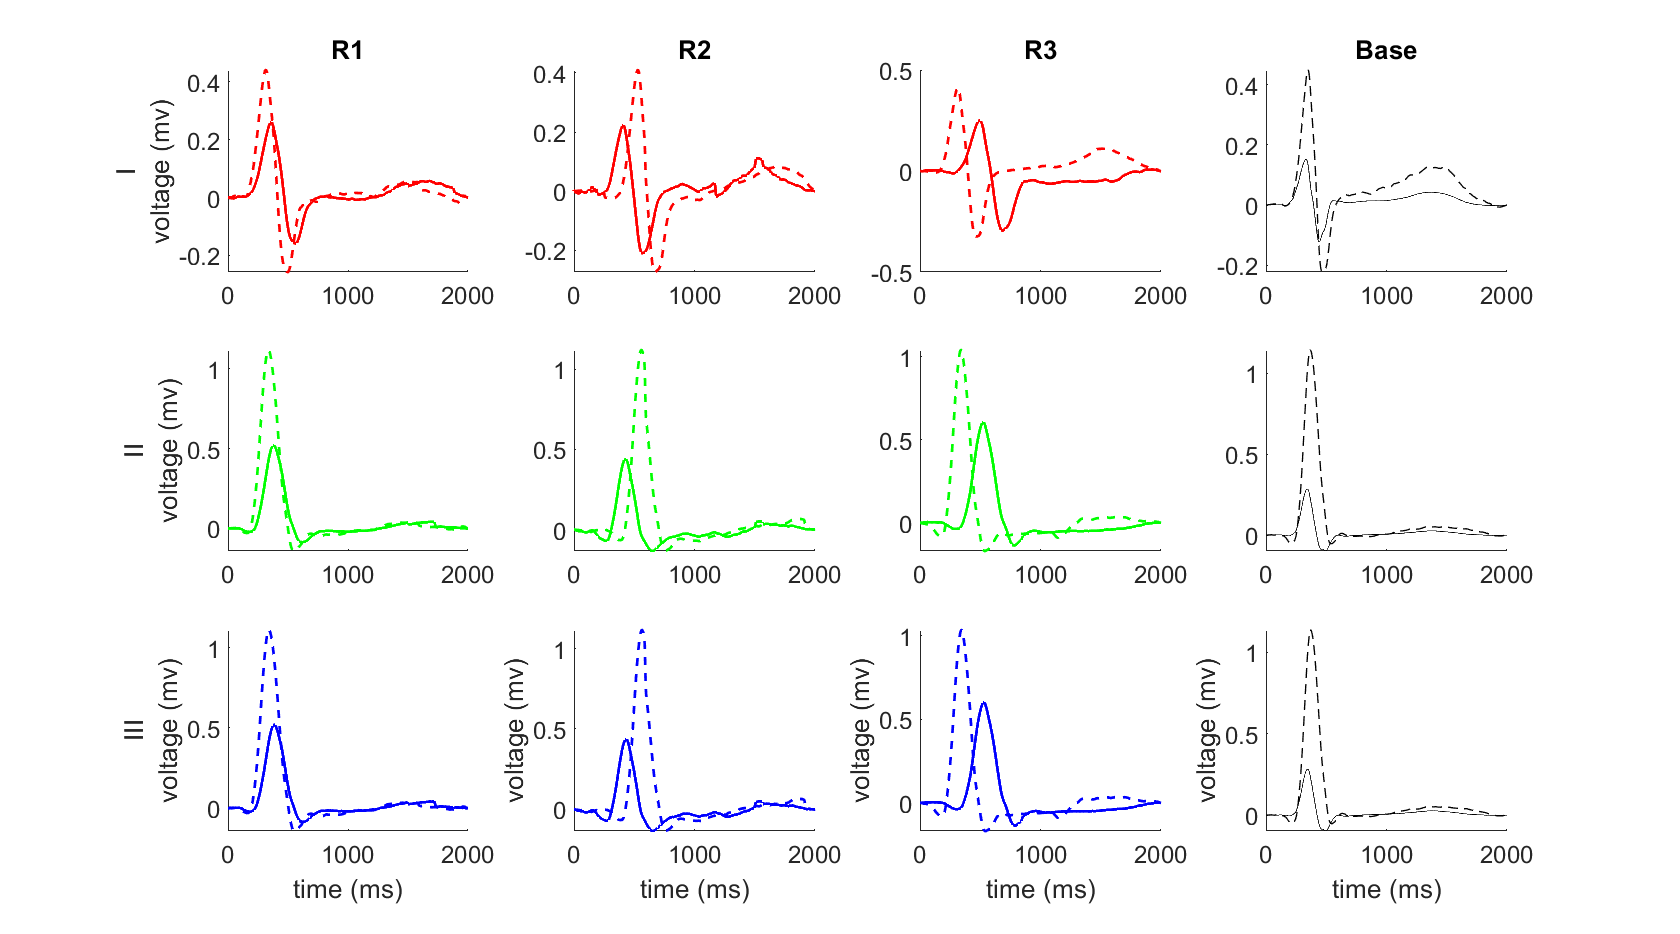
\includegraphics[width = .8\textwidth]{Figures/PostExercise.png}
	\caption{Post exercise ECG. Red: lead I, green: lead II 2, blue: lead III, Black: baseline. Column 1 from rest period 1, column 2 from rest period 2, column 3 from rest period 3. Solid lines from phase I, dashed from phase II.}
	\label{exer}
\end{figure}

\begin{figure}[H]
	
	\centering
	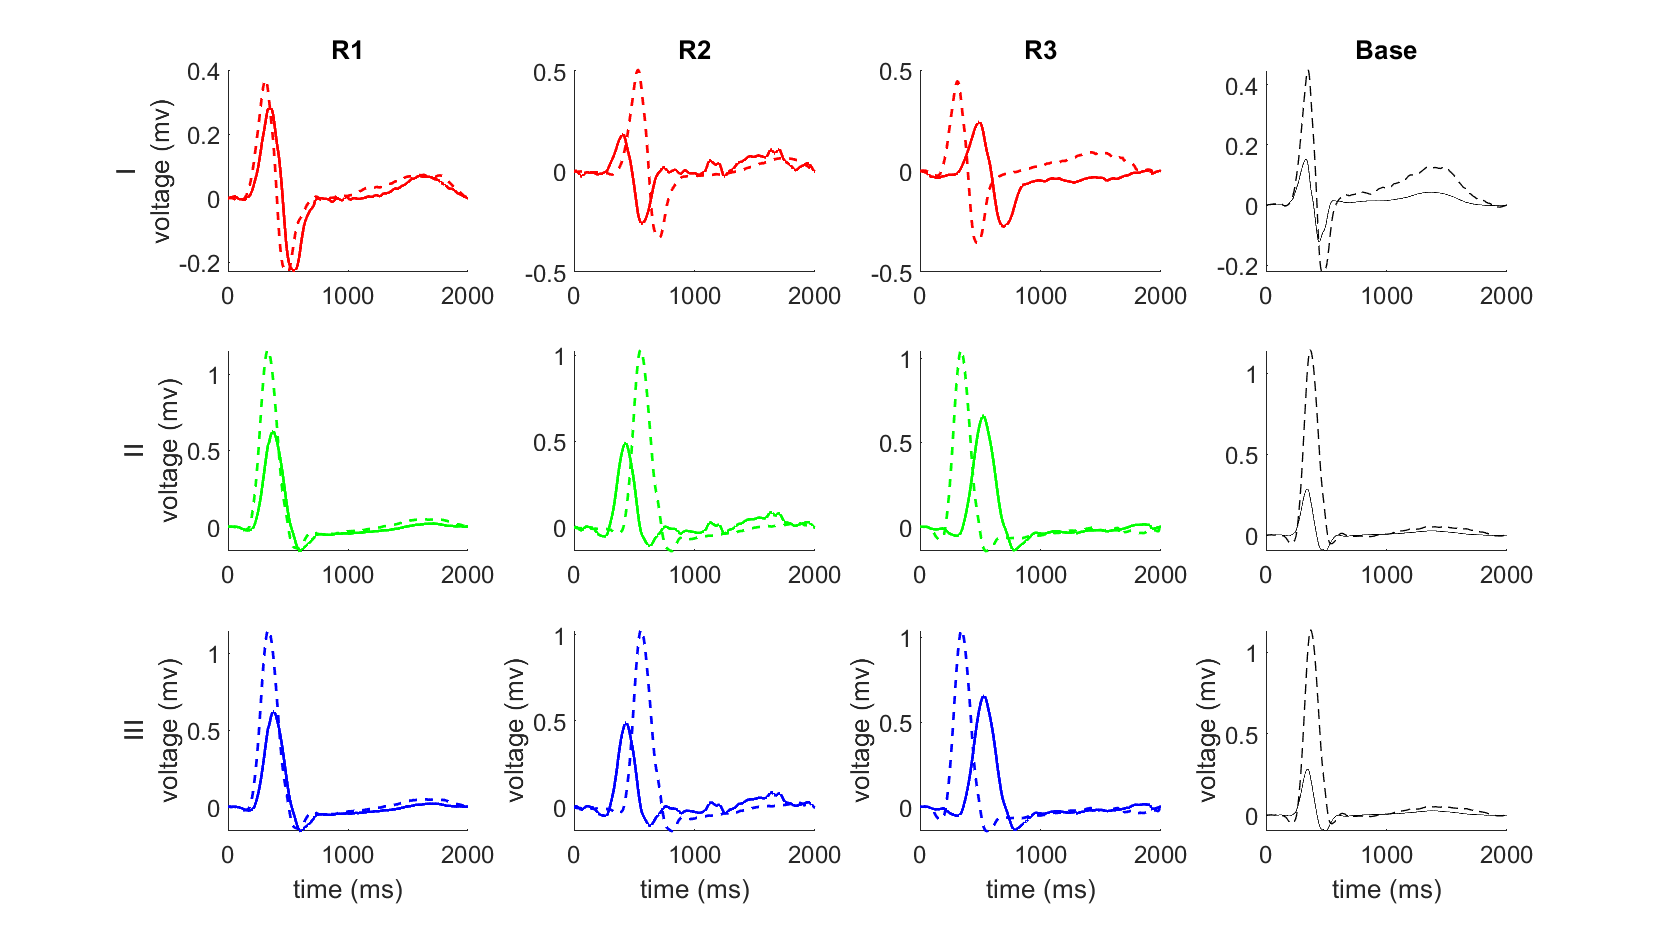
\includegraphics[width = .8\textwidth]{Figures/postrest.png}
	\caption{Post rest ECG. Red: lead I, green: lead II 2, blue: lead III, Black: baseline. Column 1 from rest period 1, column 2 from rest period 2, column 3 from rest period 3. Solid lines from phase I, dashed from phase II.}
	\label{reco}
\end{figure}


\section{Discussion}

During the first phase of this lab we measured blood pressure using a purely palpatory method, a purely ausculatory method, and a combined method. We found that the radial method was very effective for the measurement of the systolic pulse, and quite reliable but limited in that it did not allow for a diastolic measurement. On the other hand when we used the ausculatory method we found that the sounds were difficult to distinguish and as such it was only feasible to measure a semi accurate diastolic pressure. We felt that the combined method was most accurate as it combined the strengths of the two methods. It was very difficult to hear the first non laminar flow sounds that depict the systolic pressure by the ausculatory method. The first diastolic sound was the most prominent sound and to our lack of practice with the method it was the only reliable measure we could make from the ausculatory method. The palpatory method was easier to use likely due to the ease of finding a radial pulse.

During the next phase of the lab we investigated the behavior of the veins. We found that the veins on the subject's hands were unsuitable for observation however the veins on the feet were very pronounced. By using these we were able to roughly measure the venous pressure by elevating the feet above the heart until the veins very nearly collapsed (around 17 mm). Given the specific gravity of blood (1.056 g/mm) we get a value of around 1.32 mmHg for the venous pressure. This is quite a bit lower than the atrial pressure, as expected. When we press on the veins and push the blood back against the valve it causes the vein to bulge out as the blood cannot flow in retrograde against the valve.

We then moved to the exercise portion. This section was designed to investigate the effects of different intensities of exercise on the resulting recovery period. One observation to address first was the fact that the amplitude of all phase II signals (dashed lines in all ECG figures) was higher than phase I signals (solid lines in ECG figures). This is likely due to the fact that after phase I the subject was sweaty, and as such this provided better contact with the ECG electrodes, resulting in superior capture of the signal. This becomes more clear when one looks at either Figure~\ref{exer} or Figure~\ref{reco} in which the rest 3 (R3) signals for phase I and II approach a similar amplitude as the subject has perspired significantly by this point in both phase I and II. When we turn to Figure~\ref{HR} it is clear that phase I exercise was more intense than phase II, as the starting heart rate for each phase I recovery was much higher than that of phase II. Indeed the phase I exercise 2 produced the highest recorded heart rate (during rest 2 (green solid line, Figure~\ref{HR})). Additionally the phase I heart rates decayed quickly but never reached the rest heart rate of 84 bpm. The heart rates of phase I recovery did not even reach the phase II baseline of 100 bpm, showing that the intense exercise at the 180 second intervals did not allow for full recovery of the subject. An interesting trend seen across all recovery periods is an initial steep decline in heart rate followed by a less steep decline. This demonstrates that the heart is making a rapid adjustment to the cessation of exercise but is still not at a resting value. The steepness of the initial heart rate change is less in the phase II rest periods (dashed lines), and the heart rate actually approaches or crosses the baseline of 100 bpm in these periods, suggesting that at moderate exercise levels the subject was able to recover.

The changes seen in Figure~\ref{spo} are seemingly not significant. The measured \spo{} fluctuated in the high 90\% range for the duration of all recovery periods. The pulseoximeters used may have limited the resolution of this analysis due to accuracy issues. Other than the noted amplitude changes between phases there are no striking differences between any of the ECGs presented. This is in a way a good thing. We do not see any ST elevation, QRS broadening, T wave inversion, or other rhythmic changes that would be indicative of a disease state. However what is interesting is that there was an observed change in the perceived condition of the subject. The subject reported feeling much worse during the intense exercise recovery periods. Overall the results of this trial were expected. Increased intensity resulted in less recovery and a worsened perceived quality. However given a healthy subject the heart seemed to perform as expected, and no ECG, blood pressure, heart rate, or \spo{} abnormalities were found.
%%%%%%%%%%%%%%%%%% Correct Bibliography Style

\bibliography{C:/Users/Jake/Documents/library}
\bibliographystyle{IEEEtran}


\end{document}








